\subsection{OMS (Object Modeling System)}
\par
\subsubsection{Overview of OMS}
\par
OMS stands for Object Modeling System designed for environmental modeling. It is a collaborative project carried out by US Department of Agriculture and other partner organizations, which are involved in agro-environmental modeling. The OMS is a component-based software framework for environmental model development, data provisioning, testing, validation and deployment [1]. It allows the implementation of single or multiple process modules that can be developed or applied for custom-tailored module configurations [2]. With the help of the OMS framework, it is easier and more efficient for scientists to create or modify scientific models, simulate and run the models, analyze and evaluate the results. The OMS framework is an open source software system. Software developers can contribute to the OMS framework by adding new features to the existing framework to improve the performance of the framework.
\par
\subsubsection{Technical Implementation}
\par
OMS supports component based software engineering. Models and components are treated as objects in OMS. An individual component is a web service or a module that encapsulate a set of related functions separated from the surrounding framework environment [4]. The OMS framework introduces a new approach of component modeling. In OMS framework, components are normal classes enriched with Java language level annotations. A normal class consists of fields and methods, which will be supplemented by language level annotations. The annotations are used to find the entry point of data flow and method execution. The computational method of a component will have a tag “@Execute” and data flows are indicated by the tags “@In” and “@Out”.
The following example shows parts of a simple component of a bank account, whose financial credit varies year to year.
\begin{verbatim}
//1. First we have to import the necessary annotation interfaces.
import oms3.annotations.*;
import oms3.control.Iteration;

//2. We can now use the annotations imported to indicate the data flow.
@In public double withdrawal;
@In public double interest_rate;
@In public double account;
@In public int year;
@In public String output;
// 3. We can declare a computational function with the tag 
“@Execute”, which processes the data flow.
@Execute
public void compute() {
	 if (i<year){
		 int currentyear = 2012+i;
		 String s = String.format(",%1d,%2$7.2f", currentyear, account);
		 System.out.println(s);
		 w.println(s);
		 accountStatusinNextYear();
	 }
	 i++;
}
//4. The annotation “@Finalize” indicates the framework that the 
following method will be executed at last to finalize the processing 
of data flow.
@Finalize
	public void done() {
	w.close();
	}
}
\end{verbatim}
\par
The OMS framework provides simulations features to test and analyze the models, since it makes use of the advantages domain specific language, which are provided by the Groovy programming language. An OMS simulation provides all the necessary resources to run a model and it consists of following parts:
\begin{itemize}
  \item model and component executables, the core component to run and to be tested	
  \item model specific parameter to indicate the input and output of data flow
  \item some strategies for handling output	
  \item evaluate the model result with statistics or visualization
\end{itemize}
\par
The following is a part of a simple simulation file to run the model “bank account”:
\begin{verbatim}
//1. We have to import the necessary library.
import static oms3.SimBuilder.instance as OMS3
OMS3.sim (name:"Konto"){
//2. define the location of the components
	def work = "D:\\workspace_new\\OMS Model"
	resource "D:\\workspace_new\\OMS Model\\dist\\*.jar"
	model(classname:"Bankkonto.Bankkonto"){
//3. specify the input data for the components
		parameter {
		withdrawal 50
		account 	3000
		interest_rate 0.15
year 	10
		output "$work\\output.csv"
		}
	}
}
\end{verbatim}
\par
The following figure shows the result after running the simulation:
\begin{figure}[h]
	\centering
	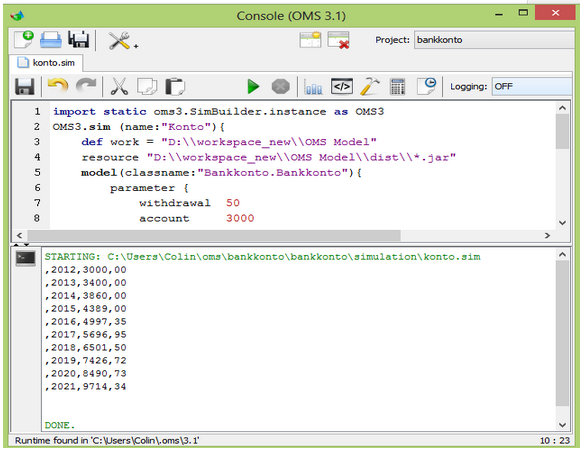
\includegraphics[width=0.7\textwidth]{pics/oms/Figure9.png}
	\caption{Result after running the model “bank account”
 \label{fig:Result_Bank_Account}}	
\end{figure}
\par
OMS also provides diagram visualization features for the simulation results for better understanding and evaluation. The following figure shows the diagram of the status changes of the bank account of different years.
\begin{figure}[h]
	\centering
	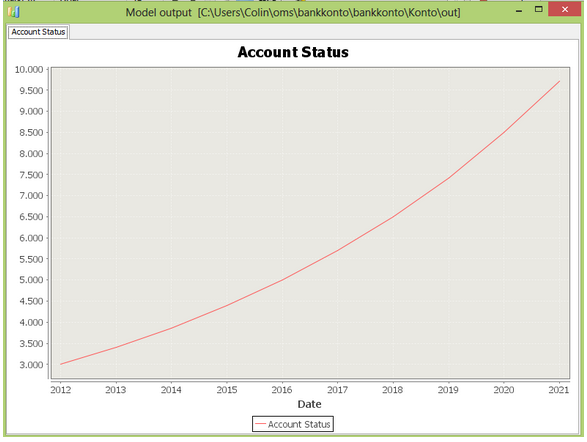
\includegraphics[width=0.7\textwidth]{pics/oms/Figure10.png}
	\caption{Visualization of the status of a bank account
 \label{fig:Visualization_Bank_Account}}	
\end{figure}
The new version of the OMS framework 3.1 supports multiple threading. Each OMS3 component will be executed in a separate thread, which is managed by the framework runtime. Thread communication happens when data flow from the “@Out” field of one component to the “@In” field of another component is carried out. The component will wait until all its necessary inputs are present and satisfied, then it starts to execute. Since modern computers are equipped with multi-core processors, the multi-threading feature will greatly make use of the power of the processors to improve the performance of the framework.
\par
\subsubsection{Advantages of OMS}
\par
The OMS framework provides the following benefits for model developers: [5]
\begin{itemize}
\item The OMS framework enables efficient transfer of technology, because of the  integration of various software tools in one platform. Due to the common modeling platform and common user interface, the OMS will reduce the start-up time of model development and lower training costs of users.

\item The OMS framework reduces the costs of developing new software technologies. With OMS, model developers can put scientific knowledge into packages as modules in OMS to build new customized software packages at a small fraction of costs.

\item Model developers are able to apply the most suitable science to a specific problem. The OMS provides various software tools for model developers. The most appropriate modules for each individual natural problem and situation will be chosen.

\item The OMS framework enhances productivity of researchers and scientists. Model developers now focus on the science module implementation, other than graphical user interface, deployment, etc, which helps to increase the productivity and quality.

\end{itemize}
\subsubsection{Disadvantages of OMS}
\par
Although the OMS framework provides various advantages for model developers, it also faces some difficulties. [5]
\begin{itemize}
\item Model developers always lack of motivation to share model code, for example, the component libraries of environmental processes, environmental models, etc. Therefore, model developers have to build their own modules repositories or contribute to the OMS module library, so that they are available for other model developers to do further developments.

\item It is hard to predict whether a modular coding structure will be accepted or not. It will take much time for model developers to pay attention to the module design, especially the input and output requirements, module structure, meta data description, and proper use of annotations. In this way, the quality and usability of the module will be guaranteed.

\item Willingness to share data sets also affects the usability of the OMS framework. The data sets mentioned here are input or output of a model, for example, data for a range of natural resource processes covering different climatic and physio graphic regions across the world. Without these data sets, it is hard to reuse an existing model, since the data is important for comparison and evaluation. Without proper comparison and evaluation, further development of the existing model is almost impossible.

\item Furthermore, it is hard to transplant models, which are developed with the OMS framework, to other framework platforms. The interoperation ability of the OMS framework is not good enough, to make the models also run on other platforms flawlessly.

\end{itemize}
